\subsection{Quattordicesimo sprint}

\begin{minipage}{\textwidth}
  Di seguito è riportata la distribuzione delle ore per ciascun membro del team, accumulate in totali per persona e per ruolo:
  \begin{table}[H]
    \begin{tabularx}{\textwidth}{|c|*{6}{>{\centering}X|}c|}
      \hline
      \multicolumn{8}{|c|}{\textbf{Consuntivo orario}} \\
      \hline
      \textbf{Membro del team} & \textbf{Re} & \textbf{Am} & \textbf{An} & \textbf{Pt} & \textbf{Pr} & \textbf{Ve} & \textbf{Totale per persona} \\
      \hline
      Riccardo Cavalli & 0 & 0 & 0 & 0 & 0 & 2 & 2 \\
      \hline
      Raul Pianon & 0 & 1 & 0 & 0 & 0 & 1 & 2 \\
      \hline
      Martina Dall'Amico & 0 & 0 & 0 & 0 & 0 & 2 & 2 \\
      \hline
      Marco Cristo & 0 & 0 & 0 & 0 & 0 & 2 & 2 \\
      \hline
      Sebastiano Lewental & 1 & 0 & 0 & 0 & 0 & 1 & 2 \\
      \hline
      Mattia Zecchinato & 0 & 1 & 0 & 0 & 0 & 1 & 2 \\
      \hline
      Tommaso Stocco & 0 & 0 & 0 & 0 & 0 & 2 & 2 \\
      \hline
      \textbf{Totale ore per ruolo} & 1 & 2 & 0 & 0 & 0 & 11 & \textbf{14} \\
      \hline
    \end{tabularx}
    \caption{Sprint 14 - Consuntivo orario}
  \end{table}
  \end{minipage}

  \begin{figure}[H]
    \centering
    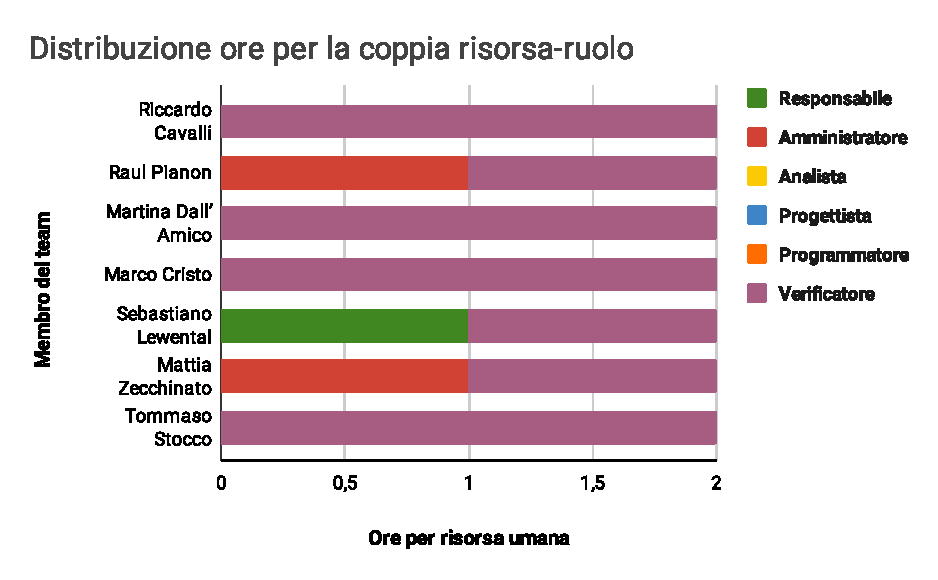
\includegraphics[width=0.90\textwidth]{assets/Consuntivo/Sprint-14/distribuzione_ore_risorsa_ruolo.pdf}
    \caption{Sprint 14 - Istogramma della distribuzione oraria per la coppia risorsa-ruolo}
  \end{figure}

  \begin{figure}[H]
    \centering
    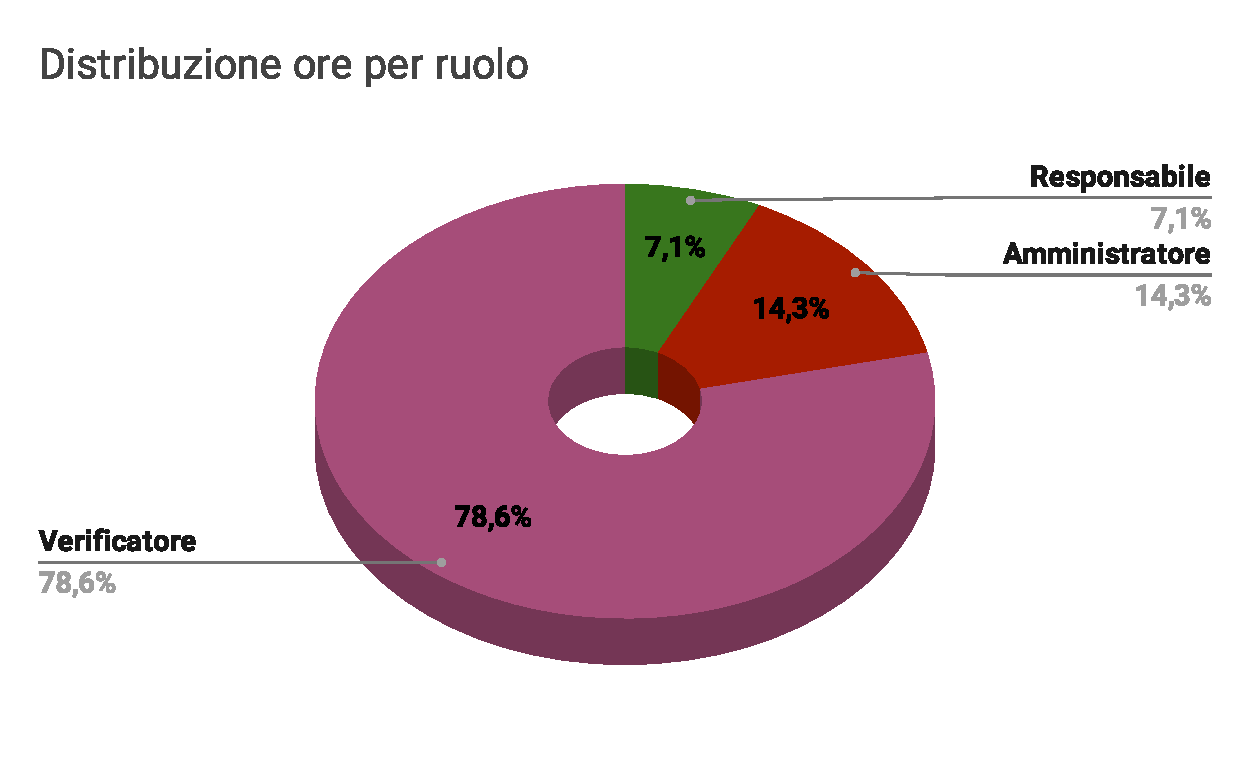
\includegraphics[width=0.90\textwidth]{assets/Consuntivo/Sprint-14/distribuzione_ore_ruolo.pdf}
    \caption{Sprint 14 - Areogramma della distribuzione oraria per ruolo}
  \end{figure}

  \begin{minipage}{\textwidth}
  Di seguito è riportato il consuntivo economico del quattordicesimo \glossario{sprint}:
  \begin{table}[H]
  \begin{adjustwidth}{-0.5cm}{-0.5cm}
    \centering
    \begin{tabular}{|P{2.9cm}|P{2.3cm}|P{2.5cm}|P{2.3cm}|>{\arraybackslash}P{2.5cm}|}
      \hline
      \multicolumn{5}{|c|}{\textbf{Consuntivo economico}} \\
      \hline
      \textbf{Ruolo} & \textbf{Ore per ruolo} & \textbf{Delta ore preventivo - consuntivo} & \textbf{Costo (in \texteuro)} & \textbf{Delta costo preventivo - consuntivo (in \texteuro)} \\
      \hline
      \Responsabile[U]{} & 1 & 0 & 30,00 & 0,00 \\ \hline
      \Amministratore[U]{} & 2 & 0 & 40,00 & 0,00 \\ \hline
      \Analista[U]{} & 0 & 0 & 0,00 & 0,00 \\ \hline
      \Progettista[U]{} & 0 & 0 & 0,00 & 0,00 \\ \hline
      \Programmatore[U]{} & 0 & 0 & 0,00 & 0,00 \\ \hline
      \Verificatore[U]{} & 11 & 0 & 165,00 & 0,00 \\ \hline
      \textbf{Totale} & \textbf{14} & 0 & \textbf{235,00} & 0,00 \\ \hline
      \textbf{Restante} & 2 & / & 35,00 & / \\ \hline
      \textbf{Sprint pregressi} & 630 & / & 12.750,00 & / \\ \hline
    \end{tabular}
    \caption{Sprint 14 - Consuntivo economico}
  \end{adjustwidth}
  \end{table}
  \end{minipage}

  \begin{figure}[H]
    \centering
    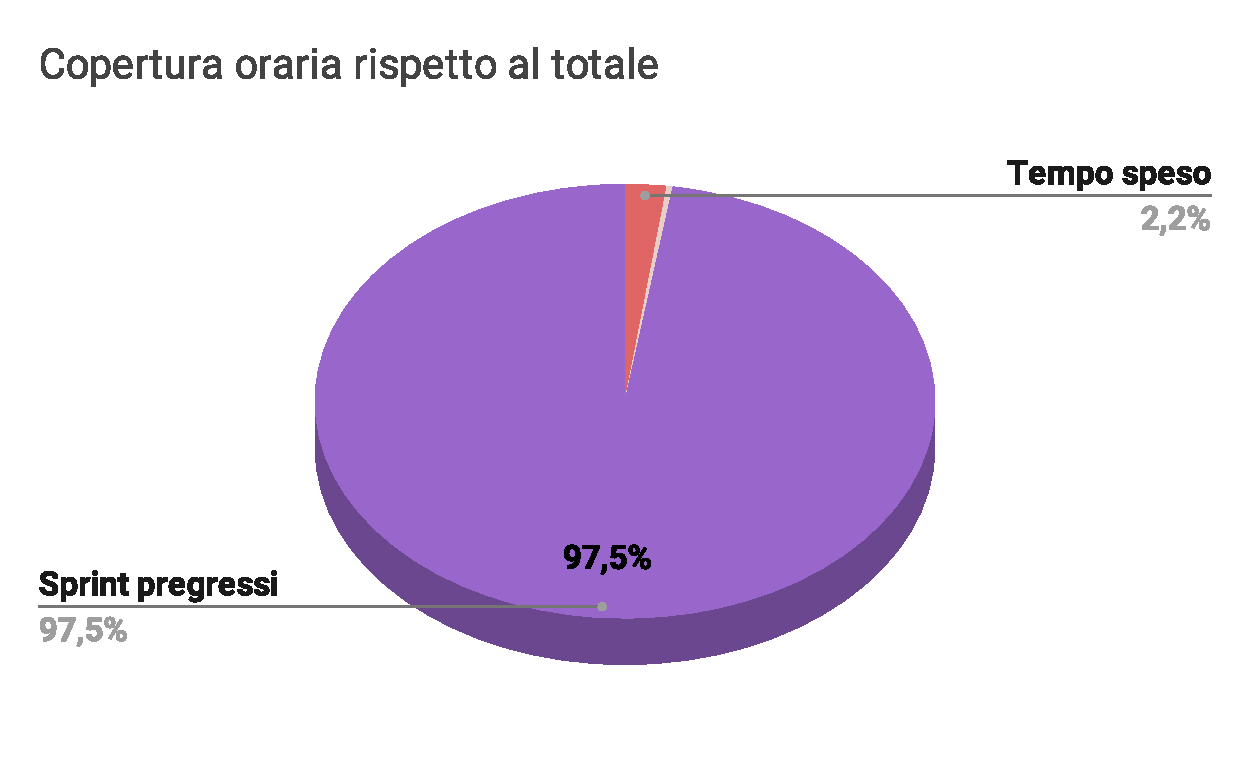
\includegraphics[width=0.90\textwidth]{assets/Consuntivo/Sprint-14/copertura_oraria.pdf}
    \caption{Sprint 14 - Areogramma del tempo speso (in ore) rispetto al totale}
  \end{figure}

  \begin{figure}[H]
    \centering
    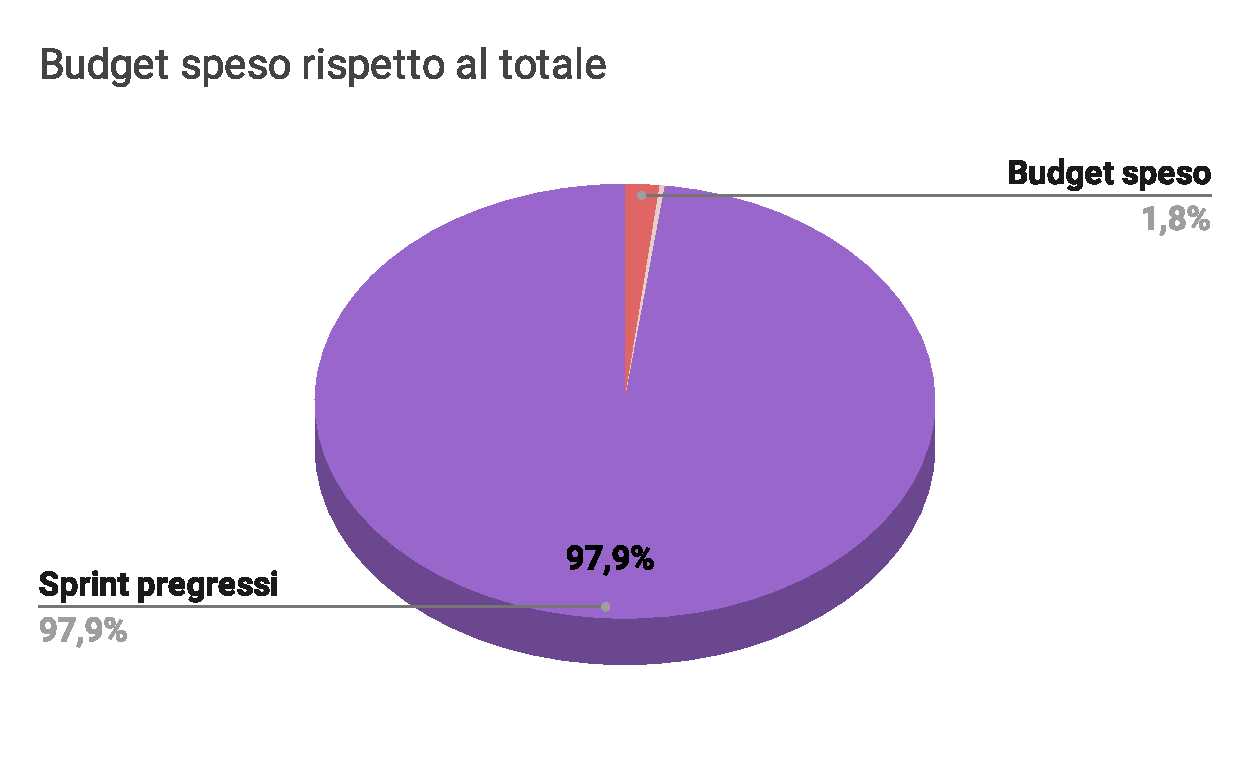
\includegraphics[width=0.90\textwidth]{assets/Consuntivo/Sprint-14/budget_speso.pdf}
    \caption{Sprint 14 - Areogramma del budget speso rispetto al totale}
  \end{figure}

  \begin{minipage}{\textwidth}
    Di seguito sono riportate le ore rimanenti per la coppia risorsa-ruolo:
    \begin{table}[H]
      \begin{tabularx}{\textwidth}{|c|*{6}{>{\centering}X|}c|}
        \hline
        \multicolumn{8}{|c|}{\textbf{Ore rimanenti per la coppia risorsa-ruolo}} \\
        \hline
        \textbf{Membro del team} & \textbf{Re} & \textbf{Am} & \textbf{An} & \textbf{Pt} & \textbf{Pr} & \textbf{Ve} & \textbf{Totale per persona} \\
        \hline
        Riccardo Cavalli & 0 & 1 & 0 & 0 & 0 & 0 & 1 \\
        \hline
        Raul Pianon & 0 & 0 & 0 & 0 & 1 & 0 & 1 \\
        \hline
        Martina Dall'Amico & 0 & 0 & 0 & 0 & 0 & 0 & 0 \\
        \hline
        Marco Cristo & 0 & 0 & 0 & 0 & 0 & 0 & 0 \\
        \hline
        Sebastiano Lewental & 0 & 0 & 0 & 0 & 0 & 0 & 0 \\
        \hline
        Mattia Zecchinato & 0 & 0 & 0 & 0 & 0 & 0 & 0 \\
        \hline
        Tommaso Stocco & 0 & 0 & 0 & 0 & 0 & 0 & 0 \\
        \hline
        \textbf{Totale ore per ruolo} & 0 & 1 & 0 & 0 & 1 & 0 & \textbf{2} \\
        \hline
      \end{tabularx}
      \caption{Sprint 14 - Ore rimanenti per la coppia risorsa-ruolo}
    \end{table}
  \end{minipage}

\subsubsection{Revisione delle attività}

Nell'arco del quattordicesimo \glossario{sprint}, il team ha svolto le seguenti attività:
\begin{itemize}
  \item Aggiornamento delle \NdP\ nelle seguenti sezioni:
  \begin{itemize}
    \item Struttura della \ST;
    \item Struttura del \MU;
    \item Test.
  \end{itemize}
  \item Aggiornamento delle funzionalità nel \MU;
  \item Consuntivo \glossario{sprint} 13;
  \item Stesura verbali interni;
  \item Aggiornamento grafici nel \PdQ;
  \item Verifica e rilascio dei seguenti documenti:
  \begin{itemize}
    \item \NdP;
    \item \PdP;
    \item \PdQ;
    \item \Gls;
    \item \MU.
  \end{itemize}
  \item Organizzazione incontro con il Professor Vardanega.
\end{itemize}

\subsubsection{Retrospettiva}

\par Di seguito sono riportati i risultati del questionario di valutazione dello \glossario{sprint}:
\begin{itemize}
  \item Organizzazione dello sprint - Valutazione: 8;
  \item Conduzione dei meeting interni - Valutazione: 8.5;
  \item Impegno e partecipazione dei singoli membri - Valutazione: 7;
  \item Tutti i membri del team erano a conoscenza delle proprie mansioni;
  \item La numerosità delle riunioni è risultata adeguata per tutti i membri del gruppo;
  \item Le riunioni sono state organizzate con il giusto preavviso;
  \item Il rapporto medio tra ore spese e ore produttive è stato inferiore a 1.5.
\end{itemize}

\vspace{0.5\baselineskip}
\par A seguire le \textbf{analisi a posteriori} del tredicesimo \glossario{sprint}:
\begin{itemize}
  \item TODO.
\end{itemize}

\subsubsection{Aggiornamento pianificazione e preventivo}
\par Il team ha definito un piano d'azione per migliorare l'organizzazione e la produttività del prossimo \glossario{sprint}:
\begin{itemize}
  \item TODO.
\end{itemize}

\paragraph*{Pianificazione futura:}
\par Con il completamento dei test di sistema e di accettazione, il team ha fissato per il prossimo \glossario{sprint} la revisione \glossario{PB}. Pertanto, il gruppo si concentrerà sulla preparazione della presentazione per il colloquio con il Professor Cardin e aggiornerà la documentazione di progetto.

\paragraph*{Preventivo "a finire" (\sezione{sec:stima_temporale}):}
\par TODO.

\paragraph*{Gestione dei rischi (\sezione{sec:analisi_rischi}):}
\par Durante il tredicesimo \glossario{sprint}, i seguenti rischi sono stati gestiti con successo:
\begin{itemize}
  \item \textbf{RO3: Sottostima delle risorse necessarie per un'attività}: TODO.
\end{itemize}
